\documentclass[12pt,a4paper,oneside,brazil]{abntex2}

% Pacotes que serão utilizados%
\usepackage{lmodern}
\usepackage[utf8]{inputenc}
\usepackage[brazil]{babel}
\usepackage[T1]{fontenc}
\usepackage{indentfirst}
\usepackage{graphicx}
\usepackage{microtype}
\usepackage{wrapfig}
\usepackage[backend = biber, style=abnt]{biblatex}
\addbibresource{Referencias.bib}

% Informações do documento %
\title{Notas Economia do Setor Público}
\author{Thiago Oliveira Coelho}
\date{\today}



\begin{document}
\pagestyle{plain}
\pagenumbering{arabic}

\maketitle
\begin{center}
Resumo baseado em \cite{rezende} e \cite{biderman} 
\end{center}
\tableofcontents
\chapter{1ª Unidade}

\section{Papel do Estado} 
As atribuições econômicas do estado segundo Musgrave:
\begin{itemize}
\item Promover ajustamentos na alocação de recursos;
\item Promover ajustamentos na distribuição de renda;
\item Manter a estabilidade econômica.
\end{itemize}

\section{Lei de Wagner}
A participação do governo aumenta junto com acréscimos de renda. HIpóteses:
\begin{itemize}
\item Bens públicos seriam bens superiores, então: $ \epsilon r_d >1$;
\item Possibilidade de surgimento de monopólios por tecnologia;
\item Crescimento da demanda por bem estar social.
\end{itemize}

\section{Efeitos Translação e concentração}
Criados por Peacock e Wiseman, sã definidos por:
\begin{itemize}
\item Translação: Choques exógenos numa nação podem mudar significativamente seu perfil de gastos e tributação;
\item Concentração: As decisões tendem a se concentrar cada vez mais na esfera federal.
\end{itemize}

\section{Falhas de mercado}
As concepções do estado moderno, em geral, atribuem a ele o papel de resolver falhas de mercado. São elas:
\subsection{Bens Públicos}
Segundo Samuelson, são públicos aqueles bens que não revelam as preferências ao serem consumidos. Por isso são não rivais e não excludentes. Geralmente são difíceis de serem distribuidos po mecanismos de mercado. São coisas como segurança, iluminação pública e justiça. Além disso, alguns intermediários entre bens públicos e privados, como saúde e educação, podem excluir pessoas de baixa renda se deixadas puramente nas mãos do mercado. Estes bens semi-públicos, caracterizados por serem não rivais e excludentes em geral possuem altíssima demanda e puca oferta; por isso podem alcançar seu equilíbrio em pontos de altíssimo preço. Eles podem ser resolvidos por duas concepções:
\begin{itemize}
\item Estado Provedor: O estado toma as rédeas da produção e distrubuição do bem, se encarregando de ofertá-lo;
\item Estado regulador: O estado fornece diretrizes e policia a iniciativa privada, que organiza a oferta do bem.
\end{itemize}

\subsection{Externalidades}
Quando a produção de algo implica em mudanças na função custo de terceiros (externalidade negativa), ou acarretam benefícios a estes (externalidade positiva).
\subsubsection{Negativa}
Nesse caso, o $Cmg$ social é maior que o privado, e a firma não lida com este custo adicional. Como $Cmg = Q^s$ a quantidade produzida será maior do que a ótima para a sociedade Por isso a solução deste tipo de externalidade é fazer com que a firma tome estes custos.

\begin{figure}[ht]
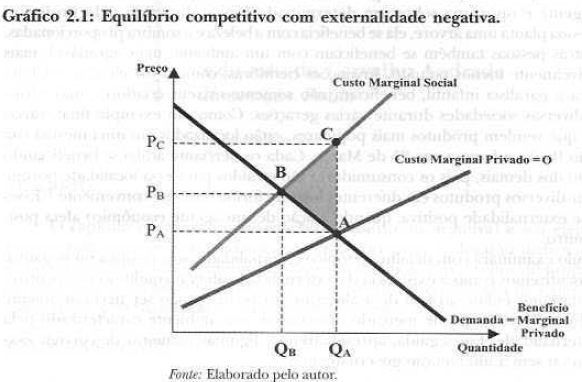
\includegraphics[scale=0.7]{Externalidade Negativa.png}
\centering
\caption{. Fonte: \cite{biderman}}
\end{figure}

Isso pode ser feito por vários métodos:
\begin{itemize}
\item Tributação;
\item Punições por meio da justiça;
\item  Regulação, por exemplo, por meio de compra de cotas para desfruto da externalidade.
\end{itemize}
\subsubsection{Positiva}
Nesse caso o benefício privado destoa do social, o que causa subprodução do bem, já que o agente produtor não internaliza os benefícios sociais.
\begin{figure}[ht]
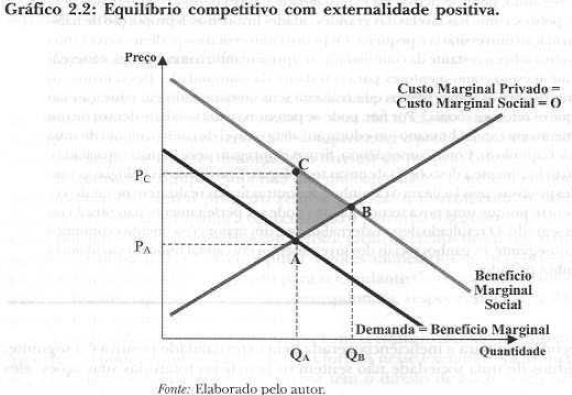
\includegraphics[scale=0.7]{Externalidade Positiva.png}
\centering
\caption{. Fonte: \cite{biderman}}
\end{figure}
Nesse caso as soluções são:
\begin{itemize}
\item Reduzir os custos, por meio de subsídios ou isenções.
\item Elevar os benefícios do agente produtor
\end{itemize}

\subsection{Poder de mercado}
\subsubsection{Monopólio}
O monopólio é caracterizado pela presença de uma única firma ofertante. Neste caso ele continua operando quando $Cmg = Rmg$ mas pelo seu poder de mercado, seu custo marginal não coincide com o preço, o que cria ineficiências (deadweight loss).
\clearpage
\begin{wrapfigure}{l}{0.5\textwidth}
	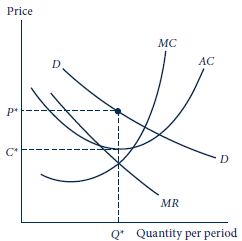
\includegraphics[width=0.4\textwidth]{Monopoly.png}
	\centering
	\caption{Fonte: \cite{nicholson}}
\end{wrapfigure}
O resultado é uma quantidade menor e preço maior do que a que ocorrerria com um mercado concorrencial, no qual $Cmg = Rmg = P$. Algumas soluções são:
\begin{itemize}
\item Leis antitruste, que evitem formação de monopólios por absorção de firmas grandes.
\item Agências reguladoras: regular a firma a fim de incentivar seu comportamento a ser mais próximo de uma firma competitiva.
\end{itemize}
\clearpage
\subsubsection{Monopólio natural}
O monopólio natural ocorre geralmente por barreiras de entrada ao mercado:
\begin{itemize}
\item Necessidade de grandes economias de escala;
\item Necessidade de grandes quantidades de capital inicial;
\item Indivisibilidade de planta;
\item Longo período de maturação;
\item Custo Fixo alto ou Custo marginal decrescente.
\end{itemize}

\begin{wrapfigure}{l}{0.5\textwidth}
	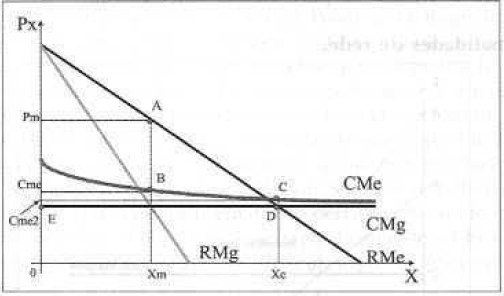
\includegraphics[width=0.4\textwidth]{Monopolio Natural.png}
	\centering
	\caption{Fonte: \cite{biderman}}
\end{wrapfigure}

É possível perceber que o equilíbrio da firma será num preço muito maior que o de mercado e numa menor quantidade. A diferença para o monopólio tradicional, é que esta firma não necessariamente está utilizando de seu poder de mercado para isso. Note que a firma está operando de modo eficiente, porém não consegue oferecer aos padrões da concorrência perfetia pelas particularidades do mercado na qual está inserido.\newline
Soluções:
\begin{itemize}
\item Estado produtor: Estatização da empresa deste setor para produção pelo setor público;
\item Estado regulador: Concessão de subsídios ou outros vantagens a fim de diminuir os custos da firma e a levar para um preço e quantidade de equilíbrio mais próximos de uma concorrência perfeita.
\end{itemize}

\subsection{Informação Assimétrica}
Configura informação assimétrica quando um dos lados da transação possui mais informações que o outro, possuindo vantagem por poder valorar melhor o bem. Supondo um mercado de informação perfeita e com produtos heterogêneos, podemos ter por exemplo uma demanda e oferta por carros usados de menor qualidade, e carros usados de boa qualdiade. Estes dois mercados estão separados, e maximizariam os excedentes, já que quem tolera carros de menor qualidade conseguem comprar exatamente estes e quem quer carros bons, vai no seu mercado específico e consegue obtê-los. Já quando pensamos em um mercado com informação assimétrica, estes dois mercados separados deixam de ter limites bem definidos, e como incerteza é imputada no preço, o novo preço de equilíbrio deste mercado conjunto será uma espécie de média ponderada dos preços dos automóveis bons e ruins. Isso irá causar um superestimação dos bens ruins e uma subestimação dos bens bons, e o produto de má qualidade tenderá a expulsar o produto de boa qualidade do mercado. \newline
Soluções:
\begin{itemize}
\item Regulação:
\begin{itemize}
\item Obrigar a parte beneficiada pela assimetria a difundir a informação que causa desnível no poder de valoração dos bens;
\item Direito de se desfazer da transação.
\end{itemize}
\item Sinalização privada:
\begin{itemize}
\item Certificações de orgãos atestanda qualidade do bem;
\item Garantia e assistência técnica, passando ao consumidor a confiança da firma naquele produto;
\item Padronização ou franqueamento para manutenção da boa imagem da marca;
\item Propaganda.
\end{itemize}
\end{itemize}

\section{Função redistributiva do estado}
O estado pode tentar promover equidade dentro da sociedade de várias formas, suponhamos que a renda do indivíduo seja determinada pelos seguintes componentes:

\[ Y_i = f(Pmg_i, \omega_i, \epsilon_i) \] 

Aonde:
\begin{itemize}
\item $Pmg$: Produtividade marginal;
\item $\omega$: Riqueza (Não confundir com renda, que é fluxo, ao contrário da riqueza que é estoque);
\item $\epsilon$: Preferência entre trabalho / prazer.
\end{itemize}

Em concorrência perfeita podemos deduzir que salário real é igual a produtividade marginal:

\[ \frac{W}{P} = Pmg\]

As medidas redistributivas que podem ser aplicadas pelo estado serão miradas nestas variáveis, já que em geral outras podem ser difíceis de quantificar e/ou influenciar. São medidas redistributivas:

\begin{itemize}
\item $Pmg$: Saúde, educação e oferta de outros bens semi-públicos que podem impactar a produtividade positivamente;
\item $\omega$: Redistribuição de riqueza por meio de reforma agrária ou imposto sobre herança por exemplo;
\item $Y$: Políticas tributárias progressivas, imposto de renda negativa, restituição de imposto de renda ou transferências de renda.
\end{itemize}

\subsection{Os problemas da redistribuição}

Basear medidas em renda monetária efetiva pode fazer o ônus recair erroneamente sobre pessoas de grande capacidade produtiva. No entanto, essa é a maneira mais simples de se desenhar programas de distribuição de renda. Além disso, temos uma literatura que diz que há custo de oportunidade entre equidade e eficiência. Para explicitar este último utilizaremos o modelo de Rawls, que tem as seguintes hipóteses:

\begin{itemize}
\item Só existem dois agentes (ou agrupamentos de agentes);
\item Só um deles trabalha;
\item Somente trabalho gera renda (não há rentistas);
\item A tributação desistimula a atividade produtiva.
\end{itemize}

A quarta hipótese é a mais importante, ela nos diz que elevados níveis de tributação desincentivam a eficiência e a capacidade produtiva da economia.

\begin{table}[h]
\centering
\begin{tabular}{|l|l|l|l|l|l|l|}
\hline
Horas trabalhadas & $Y_a$ & t(\%) & $Yd_a$ & T    & $Y_b$ & $Y_t$ \\ \hline
8                 & 8000  & 0     & 8000   & 0    & 0     & 8000  \\ \hline
7                 & 7000  & 30\%  & 4900   & 2100 & 2100  & 7000  \\ \hline
6                 & 6000  & 50\%  & 3000   & 3000 & 3000  & 6000  \\ \hline
\end{tabular}
\end{table}
A solução de Rawls será a segunda situação: o intermediário entre desigualdade e igualdade total. Há algumas críticas pertinentes ao modelo de Rawls:
\begin{enumerate}
\item Indivíduos não reduzem horas trabalhadas ao aumentar impostos:
\begin{itemize}
\item Assalariados não possuem controle sobre sua jornada de trabalho;
\item Autônomos podem não aceitar diminuição em seu padrão de vida e portanto trabalhar mais para manter a renda anterior.
\end{itemize}
\item Em países sub-desenvolvidos, aonde o fator trabalho é abundante, faz sentido redistribuir renda para as camadas mais baixas. Estas pessoas tenderão a aumentar seu consumo de bens não duráveis (como alimentos e vestimentas) e como estes bens são intensivos em trabalho, isso aumenta a demanda pelo fator.
\item A adoção de medidas redistributivas faz sentido também em mercados de trabalho aonde há discriminação. Um mercado é caracterizado como discriminatório se salários diferentes são ofertados para pessoas igualmente produtivas, e a razão explicativa desta diferença salarial se dá por fatores não-produtivas (sexo, cor de pele etc...). Neste caso, teríamos um mercado aonde os agentes discriminados ganhariam menos que sua produtividade:
\[ \frac{W}{P} < Pmg \]
O que desistimula o investimento por qualificação por parte do grupo discriminado. A transferência de renda, neste caso, complementaria o salário para que este se aproximasse da produtividade marginal do indivíduo.
\[ \triangle Y + \frac{W}{P} = Pmg \]
\end{enumerate}

\section{Função estabilizadora}
O estado também se propõe a promover o crescimento sustentável da economia, visto a natureza cíclica desta, pode aliviar os impactos destas variações, o que pode inclusive melhorar as expectativas dos agentes. 
\subsection{Políticas para aumento de demanda agregada}
Para isso pode-se utilizar de várias políticas que influenciam diferentes variáveis da demanda agregada:
\begin{itemize}
\item Políticas de renda: Em geral visam manipular os preços dos bens e os salários dos agentes $ \rightarrow C \uparrow$;
\item Política monetária: Visa manipular as taxas de juros e estoque de moeda $ \rightarrow I \uparrow$;
\item Política cambial: Visa aumentar o superávit na balança comercial $ \rightarrow (X - M) \uparrow$, tem várias formas:
\begin{itemize}
\item Câmbio fixo: O banco central dita o valor do câmbio;
\item Câmbio flutuante: O banco central deixa o câmbio variar a vontade;
\item Banda câmbial: O banco central estabelece margens aceitáveis para o valor do câmbio, e quando este ultrapassa estas margens, o banco central age para retornar o valor para dentro dos padrões. Muitos países não admitem que fazem bandas câmbiais, eles possuem câmbio flutuante, mas o banco central ainda intervine se julgar necessário, chamamos isto de \emph{flutuação suja}.
\end{itemize}
\end{itemize}
\subsection{O que é um imposto?}
Existe uma diferença entre receitas não vinculadas e receitas vinculadas:
\begin{itemize}
\item Receita vinculada: Sua transferência de recursos é direcionada para um serviço específico. EX: Taxas e contribuições de melhoria;
\item Receita não-vinculada: Sua transferência não implica uso em nenhuma área específica. EX: Impostos.
\end{itemize}
\subsection{Política fiscal}
A política fiscal é a junção das políticas tributária e orçamentária:
\begin{itemize}
\item Política tributária: Arrecadação $\rightarrow T$;
\item Política orçamentária: Despesas $\rightarrow G$;
\item Política fiscal: $\rightarrow G - T$.
\end{itemize}
Podemos classificar a política fiscal em:
\begin{itemize}
\item Se $G - T > 0 \rightarrow$ Expansionista;
\item Se $G - T < 0 \rightarrow$ Contracionista;
\item Se $G - T = 0 \rightarrow$ Equilibrada;
\end{itemize}
Teorema do orçamento equilibrado de Haavelmo:
\[ Mx G > MX T \Rightarrow \frac{dy}{dG} > \frac{dy}{dT}\]
Mesmo num governo em que se pratica política fiscal equilibrada, se em $t + 1$ o estado aumenta tanto $G$ quanto $T$ na mesma proporção, esta pode ser considerada uma politica fiscal expansionista. Isso se dá pois o multiplicador de gastos do governo é, na maior parte das vezes, maior que o multiplicador dos tributos, o que faz com que o ganho líquido seja positivo. A lógica vale também para diminuição dos gastos e tributos política equilibrada: o multiplicador negativo dos gastos governamentais terá maior impacto que o multiplicador de valor positivo de diminuição dos tributos.
\[ Mx G = \frac{1}{1-c}\]
\[ Mx T = \frac{c}{1-c}\]
\[ 0 \leq c \leq 1\]
No limite, c é igual a 1 e portanto os multiplicadores se cancelam.
\section{Objetivo da intervenção governamental}
A intervenção governamental, em geral, pode ser justificada quando age para maximizar o bem estar social:
\[  W_t = \sum^{n}_{i = 1} W_{it} \]
Pensando no bem estar individual:
\[ W_i = f(C_i, A_i, L_i, G, W_j, N_i) \]
O bem estar individual pode ser descrito como uma função de vários parâmetros. Em ordem: consumo individual, ativos individuais, lazer desfrutado individual, bens públicos consumidos, bem estar do próximo e fatores intangíveis individuais.

\section{Princípios da tributação}
\begin{itemize}
\item Adequação: Diferentes níveis de governo devem ter receitas compatíveis com suas funções e responsabilidades; 
\item Adaptabilidade: Sistema tem de ser flexível a ponto de permitir reajustes por parte da arecadação da união de acordo com as necessidades de política econômica;
\item Produtividade: Poucos tributos com elevada elasticidade de renda [Alta capacidade de arrecadação];
\item Universalidade: Obrigações tributárias devem ser exigidas sobre todos que se enquadram na base de incidência;
\item Neutralidade: Não se deve alterar os preços relativos da economia. [Ótimo de pareto fica implícito como hipótese];
\item Equidade: Assegurar qe indivíduos iguais tenham mesmo tratamento ("equidade horizontal"), e indivíduos diferentes tenham tratamentos diferentes ("equidade vertical"). Podemos usar dois critérios para classificar os indivíduos:
\begin{itemize}
\item Critério de benefício: Cobrar de acordo com o benefício marginal de cada um $ T_i = Bmg$ [Por exemplo com taxas]. Há grandes dificuldades de implementação deste tipo de critério, visto que consumidores de bens públicos não revelam suas preferências 
\item Critério da capacidade de contribuição: Cobrar de acordo com a capacidade que cada um tem de contribuição.
\end{itemize}
\end{itemize}

\subsection{Progressividade}
Um sistema tributário progressivo é aquele cuja \emph{carga tributária aumenta quanto maior a renda do contribuidor}. Sendo carga tributária:
\begin{equation} \label{Carga Tributária}
Carga = \frac{Tributos}{Renda}
\end{equation}
São as três classificações por progressividade:

\begin{figure}[h]
\centering
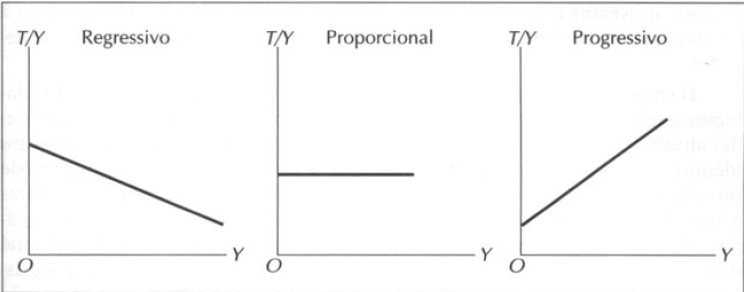
\includegraphics[scale=0.7]{Progressividade.png}
\caption{Fonte : \cite[p. 165]{rezende}}
\end{figure}

Em geral a progressividade pode ser vista como algo positivo no contexto da eficiência também, já que a utilidade marginal da renda seria decrescente, portanto seria um aumento no bem estar da sociedade se renda fosse transferida para pessoas com maior utilidade marginal. Essa hipótese pode ser criticada no sentido de que:
\begin{enumerate}
\item Essencialidade é subjetiva e subjeita a normais sociais e mudanças tecnológicas;
\item Pessoas diferentes possuiriam curvas de utilidade diferentes;
\item Algumas pessoas podem atribuir utilidades muito acima da média para certos bens supérfluos.
\end{enumerate}

\subsection{Tipos de tributo}
Temos dois modos de definirmos o valor de um tributo:
\begin{enumerate}
\item Unitário: valor fixo cobrado por unidade;
\item Ad Valorem: taxa percentual que incide sobre preço do produto.
\end{enumerate}

No caso do tributo unitário, este descloca a curva de $Cmg$ e consequentemente a oferta, em seu valor unitário $T$. Já no caso do tributo Ad Valorem, este irá aumentar a inclinação da curva de $Cmg$, já que :
\[ \frac{d C}{d Q} = Cmg + T \]

Considerando o preço do produto com tributos como:
\[ P = C + T\]
Podemos ter um tributo por dentro, que incide sobre $C$:
\[ P = C + t C \Rightarrow P = C ( 1 + t) \]
Perceba que neste caso o aumento no preço é exatamente igual a alíquota, diferentemente do tributo por fora, que incide sobre $P$:
\[ P = C + t P \Rightarrow P ( 1 + t ) = C \Rightarrow P = \frac{C}{1 + t}\]
Perceba a semelhança com o multiplicador. Este tipo de tributo acaba tendo alíquota efetiva maior do que a estabelecida. 

\chapter{2ª Unidade}
\label{cha:2_unidade}




\printbibliography
\end{document}